% !TeX root = thesis.tex

\chapter{Software Engineering}
\label{chap:software-engineering}
The Institute of Electrical and Electronics Engineers \texttt{[IEEE]} defines the practice of Software Engineering as: "Application of a systematic, disciplined, quantifiable approach to the development, operation and maintenance of software; that is, the application of engineering to software" \cite[p.~421]{8016712}. The word ``systematic'' in this definition, emphasises the need for a structured process, depicting guidelines and models that describe how software should be developed the most efficient way possible. Such a process does exist and it is often referred to as the Software Development Life Cycle (SDLC) \cite[p.~420]{8016712}. In the absence of a model, i.e. when the developer does what they deem correct without following any rules, the term \emph{Cowboy coding} is used \cite[p.~34]{landry2011iterative}.

% !TeX root = ../thesis.tex

\section{Software Development Life Cycle}\label{sec:se-sdlc}
An implementation of the SDLC consists of two parts. The first part is a list of phases, and the second part is a function that describes the transitions between these phases. Depending on the nature of the software, existing phases can either be omitted or additional phases can be added. The five phases below were compiled from multiple sources \cite{2010govardhan, 7106435} and describe a generic approach to which most software projects adhere.
\begin{enumerate}
	\bolditem{Requirements phase} In the first phase of the development process, the developers acquaint themselves with the project and compile a list of the desired functionalities \cite{7106435}. Subsequently, the developers can decide on the financial details, the required hardware specifications as well as which external software libraries will need to be acquired.
	
	\bolditem{Design phase} After the developer has gained sufficient knowledge about the project requirements, they can use this information to construct an architectural design of the application. This design consists of multiple documents, such as user stories and UML-diagrams. A user story describes which actions can be performed by which users, whereas a UML-diagram specifies the technical interaction between the individual components.
	
	\bolditem{Implementation phase} In the third phase, the developers will write code according to the specifications defined in the architectural designs.
	
	\bolditem{Testing phase} The fourth phase is the most critical. This phase will require the developers and quality assurance managers to test the implementation of the application thoroughly. The goal of this phase is to identify potential bugs before the application is made available to other users.
	
	\bolditem{Operational phase} The final phase marks the completion of the project, after which the developers can integrate it into the existing business environment of their customer.
\end{enumerate}

\noindent After we have identified the phases, we must define the transition from one phase into another phase using a model. Multiple models exist in the literature \cite{2010govardhan}, with each model having its advantages and disadvantages. This thesis will consider the traditional model, which is still widely used as of today. The base of this model is the Waterfall model by Benington  \cite{united1956symposium}. Similar to a real waterfall, this model executes every phase in cascading order. However, this imposes several restrictions. The most prevalent issue is the inability to revise a design decision when performing the actual implementation. To mitigate this problem, Royce has proposed an improved version of the Waterfall model \cite{Royce:1987:MDL:41765.41801}, which does allow a phase to transition back to any preceding phase. \Cref{fig:waterfall-royce} illustrates this updated model.

\begin{figure}[htbp!]
	\includegraphics[width=\textwidth]{assets/tikz/waterfall-model.tikz}
	\caption{Improved Waterfall model by Royce}
	\label{fig:waterfall-royce}
\end{figure}

\noindent The focus of this thesis will be on the implementation and testing phases, as these are the most time-consuming phases of the entire process. The modification that Royce has applied to the Waterfall model is particularly useful when applied to these two phases in the context of \emph{software regressions} \cite{10.1007/978-3-540-77966-7_18}. We employ the term ``regression'' when a feature that was once working as intended is suddenly malfunctioning. The culprit of this problem can be a change in the code, but this behaviour can also have an external cause, such as a change in the system clock due to daylight saving time. Sometimes, a regression can even be the result of a change to another, seemingly unrelated part of the application code \cite{6588537}.

\subsection{Taxonomy of test cases}

Software regressions and other functional bugs can ultimately incur disastrous effects, such as severe financial loss or permanent damage to the reputation of the software company. The most famous example in history is without any doubt the explosion of the Ariane 5-rocket, which was caused by an integer overflow \cite{581900}. In order to reduce the risk of bugs, we should be able to detect malfunctioning components as soon as possible to warden the application against potential failures before they occur. Consequently, we must consider the testing phase as the most critical phase of the entire development process and therefore include sufficient test cases in the application. The collection of all the test cases in an application is referred to as the \emph{\gls{testsuite}}. We can distinguish many different types of test cases. This thesis will consider three categories in particular.

\subsubsection{Unit tests}
This is the most basic test type. The purpose of a unit test is to verify the behaviour of an individual component \cite{whittaker2000}. As a result, the scope of a unit test is limited to a small and isolated piece of code, e.g. one function. Implementation-wise, a unit test is typically an example of a \gls{whiteboxtest} \cite[p.~12]{6588537}. The term white-box indicates that the creator of the test case can manually inspect the code before constructing the test. As such, they can identify necessary edge values or corner cases. Common examples of these edge values include zero, negative numbers, empty arrays or array boundaries that might cause an overflow. Once the developer has identified the edge cases, they can construct the unit test by repeatedly calling the function under test, each time with a different (edge) argument value, and afterwards verifying its behaviour and result. These verifications are referred to as \emph{assertions}. \Cref{lst:se-unit-test} contains a unit test written in Java using the popular JUnit test framework.\\
	
\lstinputlisting[caption=Java unit test in JUnit., label=lst:se-unit-test, language=Java]{assets/listings/example-unit-test.java}

\clearpage

\subsubsection{Integration tests}
The second category involves a more advanced type of tests. An integration test validates the interaction between two or more individual components \cite{whittaker2000}. Ideally, accompanying unit tests should exist that test these components as well. As opposed to the previous unit tests, a developer will usually implement an integration test as a \gls{blackboxtest} \cite[p.~6]{6588537}. The difference between a black-box and a white-box test is that a black-box test assumes that the implementation details of the code under test are unknown during the construction of the test. Since a black-box test does not require any details about the code, we can, in fact, construct the integration tests before we implement the actual feature itself. A typical example of an integration test is the communication between the front-end and the back-end side of a web application. Another example is illustrated in \Cref{lst:se-integration-test}.\\
	
\lstinputlisting[caption=Java integration test in JUnit., label=lst:se-integration-test, language=Java]{assets/listings/example-integration-test.java}

\clearpage

\subsubsection{Regression tests}
After a developer has detected a regression in the application, they will add a regression test \cite[p.~372]{8016712} to the test suite. This regression test must replicate the exact conditions and sequence of actions that have triggered the failure. The goal of this test is to prevent similar failures to occur in the future if the same conditions would reapply. An example is provided in \Cref{lst:se-regression-test}.\\

\lstinputlisting[caption=Java regression test in JUnit., label=lst:se-regression-test, language=Java]{assets/listings/example-regression-test.java}
% !TeX root = ../thesis.tex

\section{Agile Software Development}
% !TeX root = ../../thesis.tex

\subsection{Agile Manifesto}
Since the late 1990s, developers have tried to reduce the time occupied by the implementation and testing phases. As a result, several software pioneers have proposed new implementations of the SDLC, which were later collectively referred to as the \emph{Agile development methodologies}. This term was coined during a meeting of seventeen prominent software developers, in which they have defined the following four fundamental values of Agile development in the \emph{Agile Manifesto} \cite{beck2001agile}.

\begin{enumerate}
	\item \emph{Individuals and interactions} over processes and tools.
	\item \emph{Working software} over comprehensive documentation.
	\item \emph{Customer collaboration} over contract negotiation.
	\item \emph{Responding to change} over following a plan.
\end{enumerate}

\noindent According to the authors, we should interpret these values as follows: ``While there is value in the items on the right, we value the items on the left more'' \cite{beck2001agile}. When we examine these values more closely, we can observe that they all share a common philosophy, which is that software engineering should be a fast process in which communication and a short feedback loop is critical to avoid missteps. Since 2001, a variety of different programming models have arisen, each incorporating these agile principles in their own way. The most remarkable new practice is \acrfull{tdd}. Recall that an integration test is a black-box test and that as such, we can actually construct the test case in advance and write the implementation afterwards. This concept is also prevalent in TDD. This practice depicts that if we want to extend the functionality of the application, we should first modify the test cases (or add new test cases) and then modify the application code until every test case is passing \cite{10.5555/579193}.
% !TeX root = ../../thesis.tex

\subsection{The need for Agile}
In the wake of the world economic crisis, software companies were forced to devote efforts into researching how their overall expenses could be reduced. This research has concluded that in order to reduce financial risks, the \emph{time-to-market} of an application should be as short as possible. In order to accomplish this, further research was conducted, resulting in an increase of attention for agile methodologies in scientific literature \cite{ionel2009}. As was previously described in \autoref{sssec:agilevalue-workingsoftware}, agile methodologies strive to deliver a minimal version as soon as possible, allowing additional functionality to be added in an incremental fashion. This effectively results in a shorter \emph{time-to-market} and lower costs, since the company can decide to cancel the project much earlier in the process.\\

\noindent In addition to a reduced time-to-market, maintaining an agile workflow has also proven beneficial to the success rate of development. A study performed by The Standish Group revealed that the success rate of agile projects is more than three times higher compared to when traditional methodologies are practised \cite[p.~7]{standish2015chaos}, as illustrated in \autoref{fig:agile-success-rate}. 

\begin{figure}[htbp!]
	\centering
	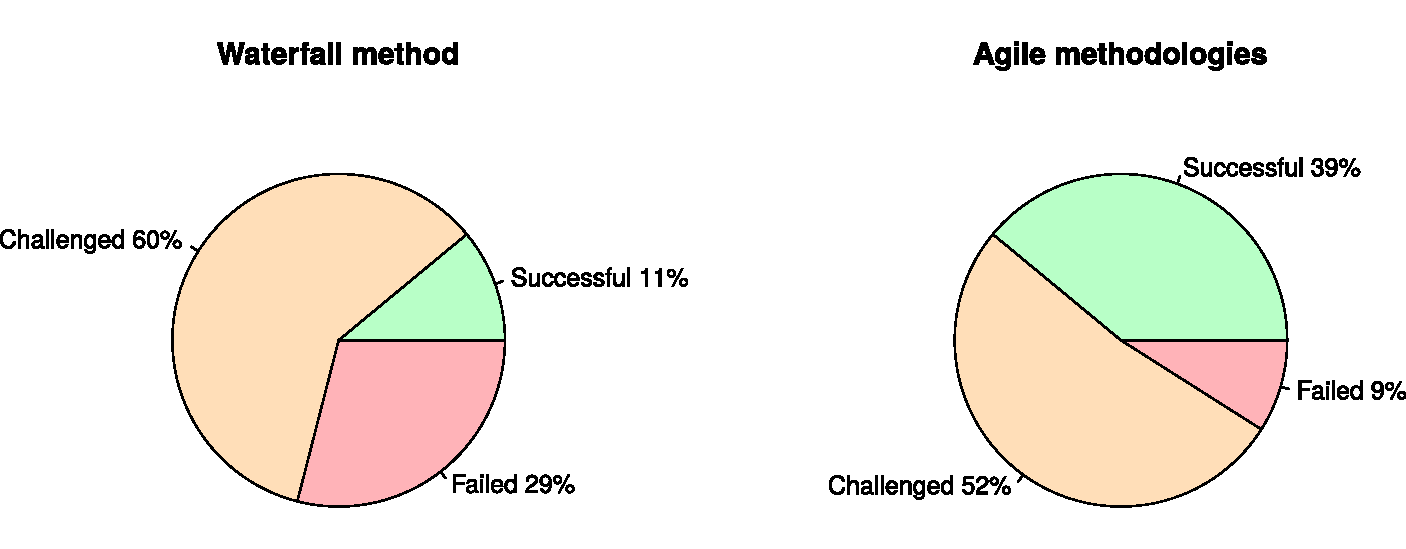
\includegraphics[width=\textwidth]{assets/agile-success-rate.pdf}
	\caption{Success rate of Agile methodologies \cite{standish2015chaos}.}
	\label{fig:agile-success-rate}
\end{figure}



%hier in hoofdstuk 7 staat iets over continuous integration
%https://link.springer.com/chapter/10.1007/978-3-319-05155-0_7

- changes moeten zeer regelmatig worden geintegreerd met elkaar -> feedback loop tussen implement -> integrate -> test -> repeat
- Continuous integration: wat?
- Bestaan aantal bestaande frameworks voor
- Maar; dat testen kan heel lang duren (zoek een bron waarin lange tests besproken worden)
- Bestaan aantal oplossingen voor -> zie volgende hoofdstuk

- feedback loop

- buildup naar waarom tooling nodig is

- waarom

- wat

- voorbeelden: Jenkins, CircleCI, Travis-CI, recent GitHub Actions + screenshots

- Probleem en oplossingen met regression tests


\section{Continuous Integration}
\subsection{Agile Manifesto}
Since the late 1990's, developers have tried to reduce the time occupied by the implementation and testing phases. In order to accomplish this, several new implementations of the SDLC were proposed and evaluated, later collectively referred to as \emph{Agile development methodologies}. The term \emph{Agile development} was coined during a meeting of seventeen prominent software developers, held between February 11-13, 2001, in Snowbird, Utah \cite{jimhighsmith2001}. As a result of this meeting, the developers defined the four key values and twelve principles that define these new methodologies, called the \emph{Manifesto for Agile Software Development}, also known as the \emph{Agile Manifesto}.\\

\noindent The four key values of Agile software development should be interpreted as follows, according to the authors: "While there is value in the items on the right, we value the items on the left more" \cite{beck2001agile}. I will explain these key values and their corresponding principles, as proposed by Kiv \cite[p.~12]{10.1007/978-3-030-03673-7_2}. It should be noted that these values are merely guidelines and that no concrete implementation is provided. A variety of different programming models, based on the agile ideologies, have arisen since 2001, each incorporating these values and principles in their own unique way.

\subsubsection{\emph{Individuals and interactions} over processes and tools}
Instead of meticulously following an outlined development process and utilising the best tools available, the main focus of attention should shift to the people behind the development and how they are interacting with each other. According to Glass, the quality of the programmers and the team is the most influential factor in the successful development of software \cite{glass2001agile}. 

\agileprinciple{5}{Build projects around motivated individuals. Give them the environment and support they need, and trust them to get the job done.}
TODO EXPLAIN

\agileprinciple{6}{The most efficient and effective method of conveying information to and within a development team is face-to-face conversation.}
TODO EXPLAIN

\agileprinciple{8}{Agile processes promote sustainable development. The sponsors, developers, and users should be able to maintain a constant pace indefinitely.}
TODO EXPLAIN

\agileprinciple{11}{The best architectures, requirements, and designs emerge from self-organizing teams.}
TODO EXPLAIN

\agileprinciple{12}{At regular intervals, the team reflects on how to become more effective, then tunes and adjusts its behavior accordingly.}
TODO EXPLAIN

\subsubsection{\emph{Working software} over comprehensive documentation}
The primary goal of software engineering is to deliver a working end product which fulfils the needs of the customer. In order to accomplish this, development should start as soon as possible. Traditional programming models demand a lot of documentation to be written prior to the actual development, which will inevitably lead to inconsistencies between the documentation and the actual application as the project grows and the requirements change \cite{Hazzan2014}. 
	
\agileprinciple{1}{Our highest priority is to satisfy the customer through early and continuous delivery of valuable software.}
TODO EXPLAIN

\agileprinciple{3}{Deliver working software frequently, from a couple of weeks to a couple of months, with a preference to the shorter timescale.}
TODO EXPLAIN

\agileprinciple{7}{Working software is the primary measure of progress.}
TODO EXPLAIN

\agileprinciple{10}{Simplicity--the art of maximizing the amount of work not done--is essential.}
TODO EXPLAIN

\subsubsection{\emph{Customer collaboration} over contract negotiation}
In traditional software engineering, the role of the customer is subordinate to the developer. Agile software engineering maintains a different perception of this role, treating both the customer and developers as equal entities. Daily contact between both parties is of vital importance to avoid misunderstandings and a short feedback loop allows the developers to cope with changes in requirements and to ensure that the customer is satisfied with the delivered product \cite{Hazzan2014}.

\agileprinciple{4}{Business people and developers must work together daily throughout the project.}
TODO EXPLAIN

\subsubsection{\emph{Responding to change} over following a plan}
The first step of the aforementioned waterfall model (\autoref{sec:se-sdlc}) was to ensure both the customer and the developers have a complete and exhaustive view of the entire application. In reality however, this has proven to be rather difficult and sometimes even impossible. As a result of this, a change in requirements was one of the most common causes of software project failure \cite{glass2001agile}. Consequently, the agile software development methodologies do not require a complete specification of the final product to be known a priori and stimulate the developers to successfully cope with changes as the application is being developed \cite{Hazzan2014}. This is accomplished by working in short iterations (sprints), instead of programming the entire application at once, which is the case with the traditional programming models.

\agileprinciple{2}{Welcome changing requirements, even late in development. Agile processes harness change for the customer's competitive advantage.}
TODO EXPLAIN

\agileprinciple{9}{Continuous attention to technical excellence and good design enhances agility.}
TODO EXPLAIN

\subsection{The need for Agile}
Over the past decade, the agile methodologies have received increasing attention amongst software developers, following the world economic crisis of 2009 \cite{ionel2009}. A consequence of this crisis was that software companies were forced to cut on their expenses and find ways to reduce the \emph{time-to-market} of their applications.

- probleem met waterfall model -> een bron hiervoor?

- feedback loop

- buildup naar waarom tooling nodig is

- waarom

- wat

- voorbeelden: Jenkins, CircleCI, Travis-CI, recent GitHub Actions + screenshots

- Probleem en oplossingen met regression tests

  - Test Case Prioritization -> Focus want geen tests weggooien
  
  - Test Suite Minimization
  
  - Test Suite Selection
  
  - Test Suite Reduction

